\documentclass[aspectratio=169]{beamer}
\usetheme{simple}

\input{preamble/preamble.tex}
\input{preamble/preamble_math.tex}
% \input{preamble/preamble_acronyms.tex}

\title{Lecture 1: Course Introduction, \\ Basics of Probability and Statistics, \\ \& A Little Bit about Contingency Tables}
\subtitle{STATS305B: Applied  Statistics II}
\author{Scott Linderman}
\date{\today}


\begin{document}


\maketitle

\begin{frame}{Introductions}

  \begin{itemize}
    \item \textbf{Instructor:} Scott Linderman (Asst. Prof., Statistics and Wu Tsai Neuro. Inst.)
    \item \textbf{TA:} Amber Hu (PhD student, Statistics)
    \item \textbf{TA:} Michael Salerno (PhD student, Statistics)
  \end{itemize}
\end{frame}

\begin{frame}{What is this course about?}

\begin{center}
    {\Large \textit{Probabilistic modeling and inference with discrete data. }}
\end{center}

\vspace{1em}

To what end? We want to:
\begin{itemize}
    \item \textbf{Predict:} given features, estimate labels or outputs
    \item \textbf{Simulate:} given partial observations, generate the rest
    \item \textbf{Summarize:} given high dimensional data, find low-dimensional factors of variation
    \item \textbf{Decide:} given past actions/outcomes, which choice is best?
    \item \textbf{Understand:} what generative mechanisms gave rise to this data?
\end{itemize}
\end{frame}


\begin{frame}{Box's Loop}
\begin{center}
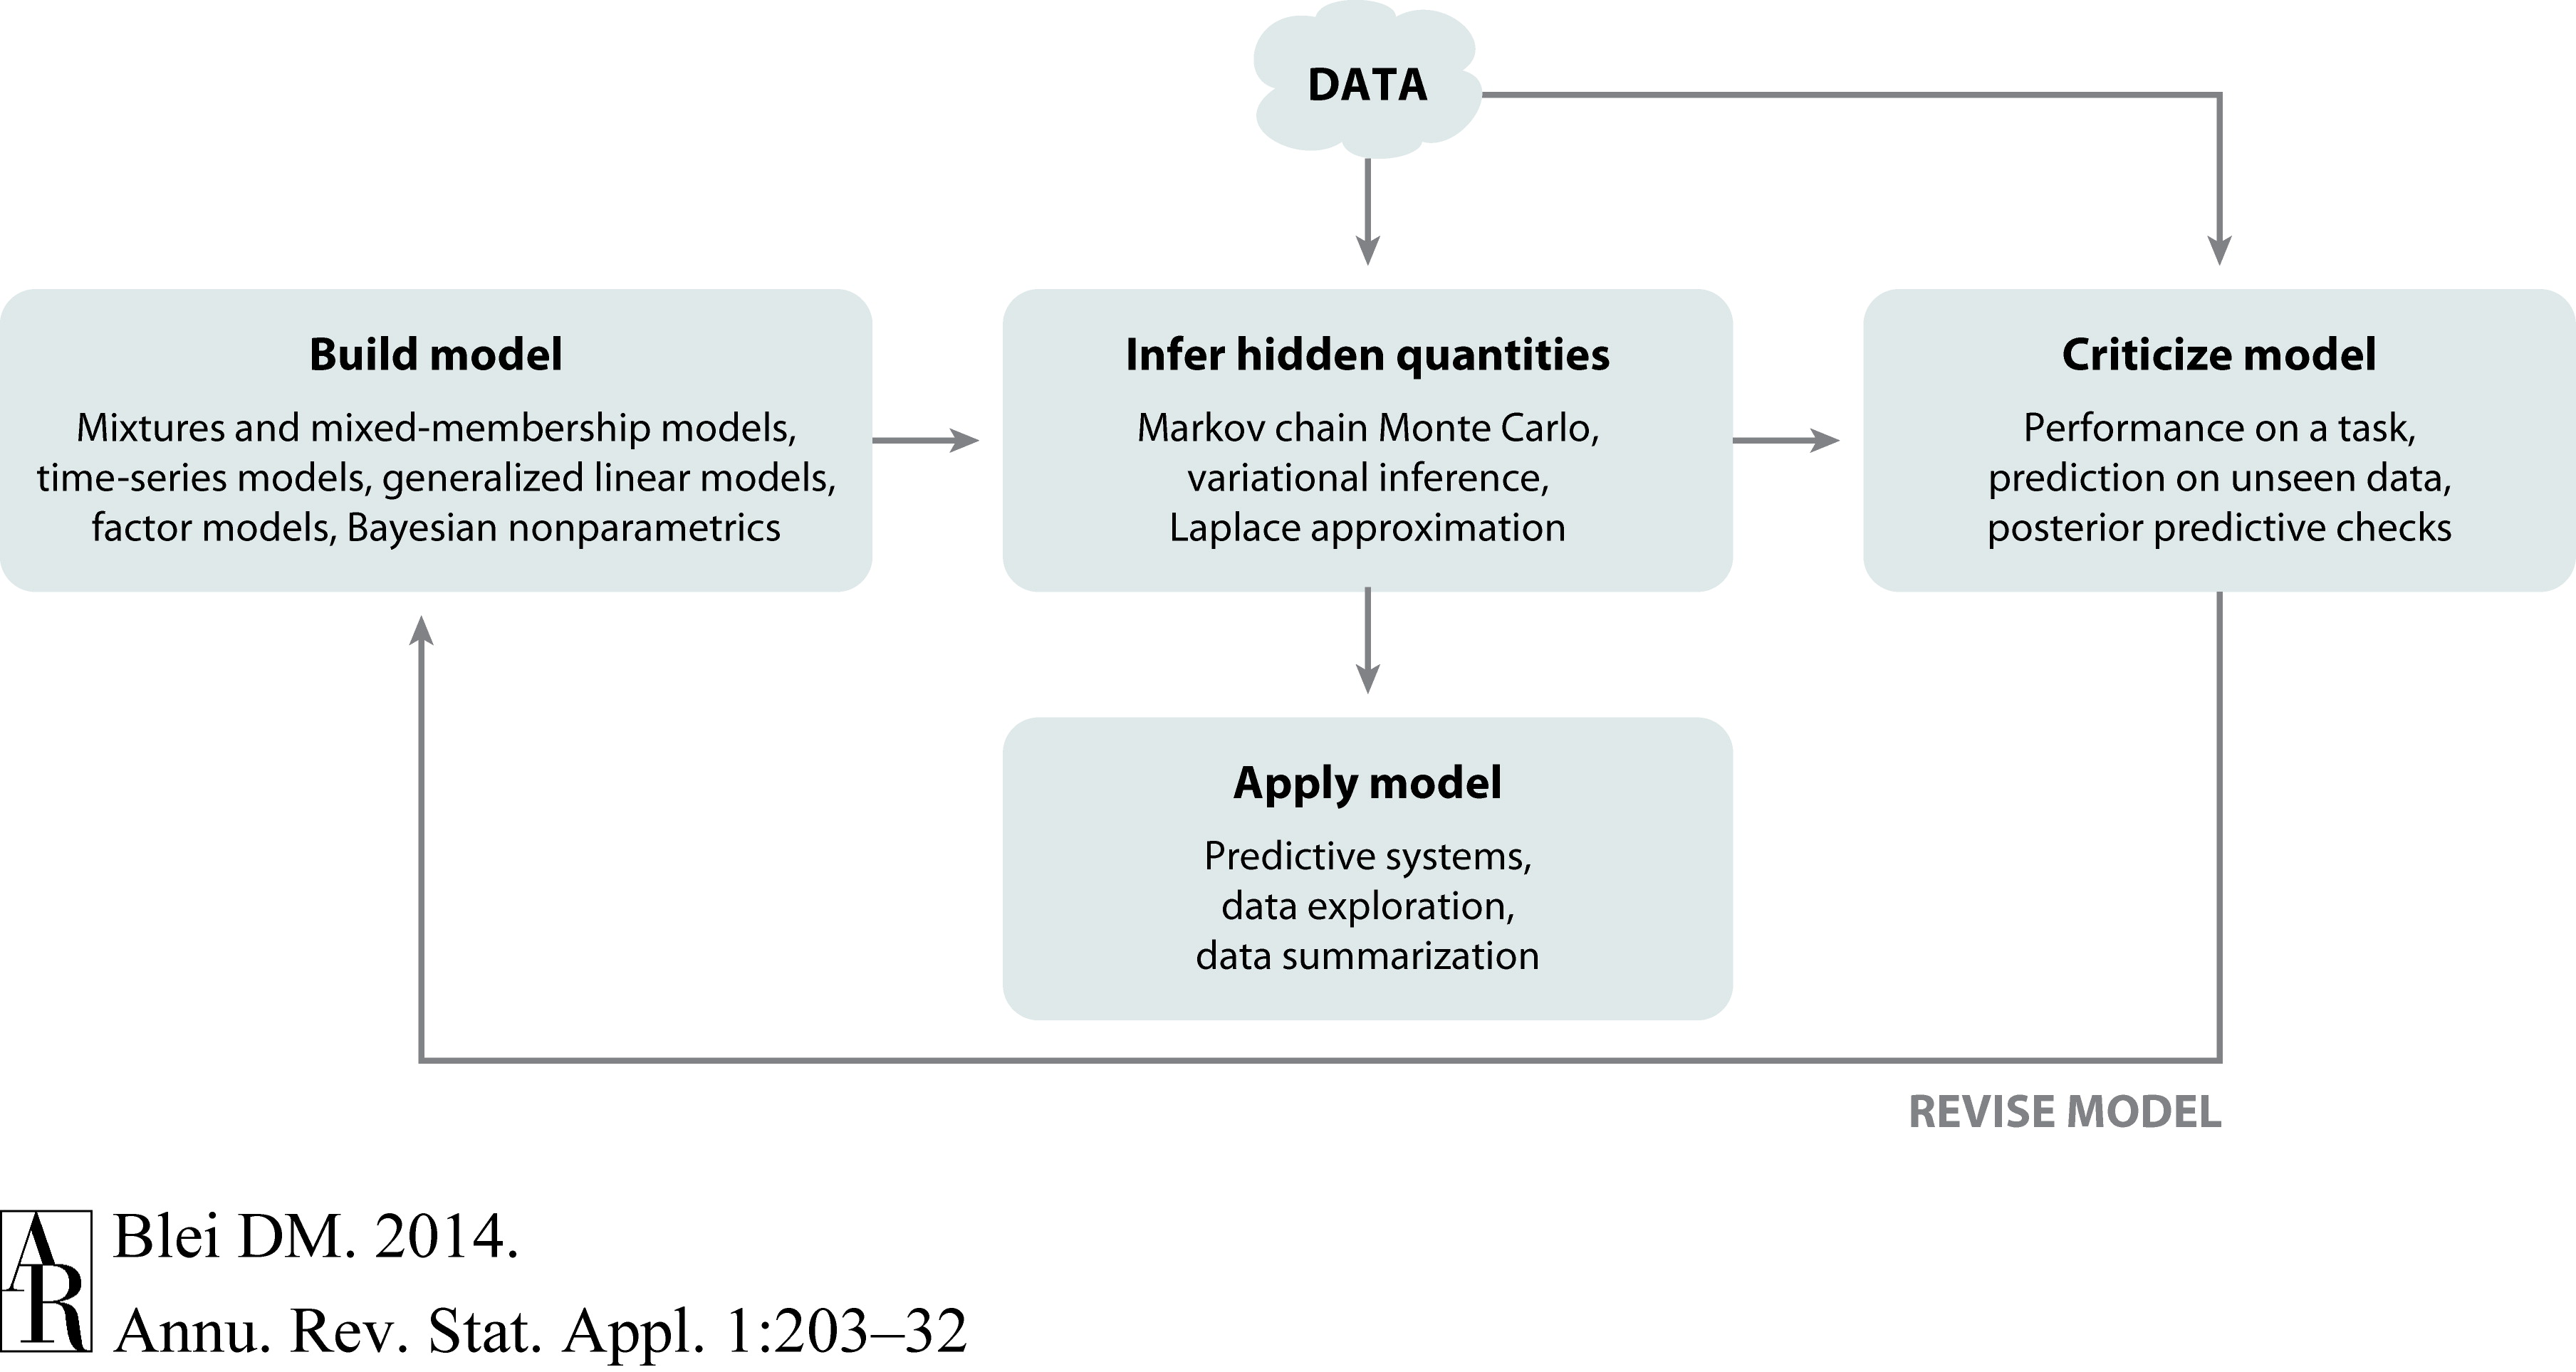
\includegraphics[width=.85\linewidth]{../lectures/figures/boxsloop.jpeg}\\
\end{center} 
\begin{flushright}
{\footnotesize \citet{Blei2014-gr}.}
\end{flushright}
\end{frame}

\begin{frame}{Course Outline}

\begin{itemize}
  \item Weeks 1-3: Classics: Exponential family distributions and GLMs
  \item Weeks 4-5: Bayesian Inference algorithms: MCMC and variational inference
  \item Weeks 6-7: Latent variable models: mixture models, HMMs, etc.
  \item Weeks 8-9: Deep generative models: VAEs, Transformers, Deep SSMs, Denoising diffusion models
  \item Week 10: Bonus: Point processes, survival analysis, etc.
\end{itemize}

\end{frame}


\begin{frame}{Learning Objectives}
  \begin{itemize}
    \item Understand the mathematical underpinnings of classical and modern models for discrete data.
    
    \item Develop expertise in an array of algorithms for parameter estimation and inference in these models.
    
    \item Be able to code these models and algorithms from scratch in Python.
  \end{itemize}
\end{frame}

\begin{frame}{Assignments}

  \begin{itemize}
    \item Weeks 1-3: Classics: Exponential family distributions and GLMs \\
    \qquad \textit{Predict outcomes of college football games with a Bradley-Terry model.}

    \item Weeks 4-5: Bayesian Inference algorithms: MCMC and variational inference \\
    \qquad \textit{Election forecasting with a Bayesian GLM.}

    \item Weeks 6-7: Latent variable models: mixture models, HMMs, etc. \\
    \qquad \textit{Changepoint detection in time series data.}

    \item Weeks 8-9: Deep generative models: VAEs, Transformers, Deep SSMs, Denoising diffusion models \\
    \qquad \textit{Build a small LLM.}

    \item Week 10: Bonus: Point processes, survival analysis, etc.
  \end{itemize}
  
\end{frame}
    

% \begin{frame}[t]{Exams}
%   \begin{itemize}
%     \item Midterm: Planning on Weds of week 5 (Feb 5).
%     \item Final: 
% \end{frame}

\begin{frame}{Logistics}

Please see the course website for the syllabus, schedule, lecture notes, grading policy, etc.

\begin{center}
  \textcolor{blue}{\url{https://slinderman.github.io/stats305b/}}
\end{center}

We will use Ed for communications, questions, etc., and Gradescope for assignments.

\end{frame}

\begin{frame}[t,allowframebreaks]{Interactive Example: College Football Playoffs}
  \label{demo-college-football-playoffs}
  
  Let's start with a hands-on example. The College Football Playoffs are
  underway, and the Super Bowl is coming up in a few weeks! If you go to a
  watch party, you might like to play the following game with your
  friends. 
  
  Before the football game starts, create a 10x10 board with the
  rows and columns numbered 0 through 9. Each cell represents a possible
  final score of the home and away team, mod 10. You and your friends
  select cells in round robin order until all 100 cells are taken. Whoever
  has the cell with the final score (mod 10) wins!

  First, let's review some basics about football... 
\end{frame}

\begin{frame}[t]{Step 1: Collect Data}
  Let's play together, using the upcoming Cotton Bowl between Ohio State
  and Texas as our example. Fill out this poll to enter your guess.
  
  \begin{center}
      \textbf{\textcolor{blue}{\url{https://tinyurl.com/stats305lec01}}}
  \end{center}
  
\end{frame}

\begin{frame}{Outline}
  \begin{itemize}
    \item Basic Probability Distributions
    \item Maximum Likelihood Estimation
    % \item Hypothesis Testing and Confidence Intervals
    \item Contingency Tables and Independence
  \end{itemize}
\end{frame}

\begin{frame}[t,allowframebreaks]{Bernoulli Distribution}
\label{bernoulli-distribution}

Toss a (biased) coin where the probability of heads is \(p \in [0,1]\).
Let \(X=1\) denote the event that a coin flip comes up heads and \(X=0\)
it comes up tails. The random variable \(X\) follows a Bernoulli
distribution, \begin{align*}
X \sim \mathrm{Bern}(p)
\end{align*}

We denote its \textbf{probability mass function (pmf)} by,

\begin{align*}
\mathrm{Bern}(x; p) 
=
\begin{cases}
p & \text{if } x = 1 \\
1 - p &\text{if } x = 0
\end{cases}
\end{align*} or more succinctly \begin{align*}
\mathrm{Bern}(x; p) = p^x (1-p)^{1-x}.
\end{align*}


The Bernoulli distribution's mean is \(\E[X] = p\) and its variance is
\(\Var[X] = p(1-p)\).
\end{frame}

\begin{frame}[t,allowframebreaks]{Binomial Distribution}\label{binomial-distribution}

Now toss the same biased coin \(n\) times independently and let
\begin{align*}
X_i &\iid\sim \mathrm{Bern}(p) \qquad \text{for } i=1,\ldots, n
\end{align*} denote the outcomes of each trial.

The number of heads, \(X = \sum_{i=1}^n X_i\), is a random variable
taking values \(X \in \{0,\ldots,n\}\). It follows a binomial
distribution, \begin{align*}
X \sim \mathrm{Bin}(n, p)
\end{align*} with pmf \begin{align*}
\mathrm{Bin}(x; n, p) = {n \choose x} p^x (1-p)^{n-x}.
\end{align*}

Its mean and variance are \(\E[X] = np\) and \(\Var[X] = np(1-p)\),
respectively.

\end{frame}

\begin{frame}[t,allowframebreaks]{Poisson Distribution}\label{poisson-distribution}

Now let \(n \to \infty\) and \(p \to 0\) while the product
\(np = \lambda\) stays constant. In that limit, the binomial distribution converges to
the Poisson distribution over non-negative integers $X \in \naturals$,
\begin{align*}
X \sim \mathrm{Po}(\lambda).
\end{align*} 
Its pmf is, \begin{align*}
\mathrm{Po}(x; \lambda) &= \frac{1}{x!} e^{-\lambda} \lambda^x.
\end{align*}

The mean and variance are both \(\lambda\). The fact that the mean
equals the variance is a defining property of the Poisson distribution,
but it's not always an appropriate modeling assumption.

\end{frame}

\begin{frame}[t,allowframebreaks]{Categorical Distribution}
\label{categorical-distribution}

Instead of a biased coin, consider a biased \emph{die} with \(K\) faces
and corresponding probabilites
\(\mbpi = (\pi_1, \ldots, \pi_K) \in \Delta_{K-1}\), where $\Delta_{K-1}$
 denotes the \((K-1)\)-dimensional simplex,
\begin{align*}
\Delta_{K-1} &= \left\{\mbpi \in \reals_+^K: \sum_k \pi_k = 1 \right\}
\end{align*} 

The outcome \(X \in \{1,\ldots,K\}\) follows a categorical distribution, 
$X \sim \mathrm{Cat}(\mbpi)$, with pmf 
\begin{align*}
\mathrm{Cat}(x; \mbpi) &= \prod_{k=1}^K \pi_k^{\bbI[x=k]}
\end{align*} 
where \(\bbI[y]\) is an indicator function that returns 1
if \(y\) is true and 0 otherwise. 

The categorical distribution is a natural generalization of
the Bernoulli distribution to random variables that can fall into more
than two categories.

Alternatively, we can represent \(X\) as a \textbf{one-hot vector}, in
which case \(X \in \{\mbe_1, \ldots, \mbe_K\}\) where
\(\mbe_k = (0, \ldots, 1, \ldots, 0)^\top\) is a one-hot vector with a 1
in the \(k\)-th position. Then, the pmf is, \begin{align*}
\mathrm{Cat}(\mbx; \mbpi) &= \prod_{k=1}^K \pi_k^{x_k}
\end{align*}

\end{frame}

\begin{frame}[t,allowframebreaks]{Multinomial Distribution}
  \label{multinomial-distribution}

From this representation, it is straightforward to generalize to \(n\)
independent rolls of the die, just like in the binomial distribution.
Let \(Z_i \iid\sim \mathrm{Cat}(\mbpi)\) for \(i=1,\ldots,n\) denote the
outcomes of each roll, and let \(X = \sum_{i=1}^n Z_i\) denote the total
number of times the die came up on each of the \(K\) faces. Note that
\(X \in \naturals^K\) is a \emph{vector-valued random variable}. Then,
\(X\) follows a multinomial distribution, \begin{align*}
X \sim \mathrm{Mult}(n, \mbpi),
\end{align*} with pmf, \begin{align*}
\mathrm{Mult}(\mbx; n, \mbpi) &= \bbI[\mbx \in \cX_n] \cdot {n \choose x_1, \ldots
, x_K} \prod_{k=1}^K \pi_k^{x_k} 
\end{align*} where
\(\cX_n = \left\{\mbx \in \naturals^K : \sum_{k=1}^K x_k = n \right\}\)
and ${n \choose x_1, \ldots, x_K} = \frac{n!}{x_1! \cdots x_K!}$ denotes the multinomial function.

The expected value of a multinomial random variable is
\(\E[X] = n \mbpi\) and the \(K \times K\) covariance matrix is,
\begin{align*}
\Cov(X) &= n 
\begin{bmatrix}
\pi_1(1-\pi_1) & -\pi_1 \pi_2 & \ldots & -\pi_1 \pi_K \\
-\pi_2 \pi_1 & \pi_2 (1-\pi_2) & \ldots & -\pi_2 \pi_K \\
\vdots & \vdots & \vdots & \vdots \\
-\pi_K \pi_1 & -\pi_K \pi_2 & \ldots & \pi_K (1- \pi_K)
\end{bmatrix}
\end{align*} with entries \begin{align*}
[\Cov[X]]_{ij} &= 
\begin{cases}
n \pi_i (1-\pi_i) & \text{if } i = j \\
-n \pi_i \pi_j & \text{if } i \neq j \\
\end{cases}
\end{align*}

\end{frame}

\begin{frame}[t,allowframebreaks]{Poisson / Multinomial
Connection}\label{poisson-multinomial-connection}

Suppose we have a collection of independent (but not identically
distributed) Poisson random variables, \begin{align*}
X_i &\sim \mathrm{Po}(\lambda_i) & \text{for } i&=1,\ldots,K.
\end{align*} Due to their independence, the sum
\(X_\bullet = \sum_{i=1}^K X_i\) is Poisson distributed as well,
\begin{align*}
X_\bullet &\sim \mathrm{Po}\left( \sum_{i=1}^K \lambda_k \right)
\end{align*} (We'll use this \(X_\bullet\) notation more when we talk about contingency tables.)

Conditioning on the sum renders the counts \emph{dependent}. (They have
to sum to a fixed value, so they can't be independent!) Specifically,
given the sum, the counts follow a multinomial distribution,
\begin{align*}
(X_1, \ldots, X_K) \mid X_\bullet = n &\sim \mathrm{Mult}(n, \mbpi)
\end{align*} where \begin{align*}
\mbpi &= \left(\frac{\lambda_1}{\lambda_\bullet}, \ldots, \frac{\lambda_K}{\lambda_\bullet} \right)
\end{align*} with \(\lambda_{\bullet} = \sum_{i=1}^K \lambda_i\). In
words, given the sum, the vector of counts is multinomially distributed
with probabilities given by the normalized rates.

\end{frame}

\begin{frame}{Outline}
  \begin{itemize}
    \item Basic Probability Distributions
    \item \textbf{Maximum Likelihood Estimation}
    % \item Hypothesis Testing and Confidence Intervals
    \item Contingency Tables and Independence
  \end{itemize}
\end{frame}


\begin{frame}[t,allowframebreaks]{Maximum Likelihood
Estimation}\label{maximum-likelihood-estimation}

The distributions above are simple probability models with one or two
parameters. How can we estimate those parameters from data? We'll focus
on maximum likelihood estimation.

The log likelihood is the probability of the data viewed as a function
of the model parameters \(\mbtheta\). Given i.i.d. observations
\(\{x_i\}_{i=1}^n\), the log likelihood reduces to a sum, \begin{align*}
\cL(\mbtheta) &= \sum_{i=1}^n \log p(x_i; \theta).
\end{align*} The maximum likelihood estimate (MLE) is a maximum of the
log likelihood, \begin{align*}
\hat{\mbtheta}_{\mathsf{MLE}} &= \arg\; \max \cL(\mbtheta)
\end{align*} (Assume for now that there is a single global maximum.)
\end{frame}

\begin{frame}[t,allowframebreaks]{Example: MLE for the Bernoulli distribution} 
Consider a Bernoulli distribution unknown parameter
\(\theta \in [0,1]\) for the probability of heads. Suppose we observe
\(n\) independent coin flips \begin{align*}
X_i &\iid\sim \mathrm{Bern}(\theta) & \text{for } i&=1,\ldots, n.
\end{align*} Observing \(X_i=x_i\) for all \(i\), the log likelihood is,
\begin{align*}
\cL(\theta) 
&= \sum_{i=1}^n x_i \log \theta + (1 - x_i) \log (1 - \theta) \\
&= x \log \theta + (n - x) \log (1 - \theta)
\end{align*} where \(x = \sum_{i=1}^n x_i\) is the number of flips that
came up heads.

Taking the derivative with respect to \(p\), \begin{align*}
\frac{\dif}{\dif \theta} \cL(\theta) 
&= \frac{x}{\theta} - \frac{n - x}{1 - \theta} \\
&= \frac{x - n\theta}{\theta (1 - \theta)}.
\end{align*} Setting this to zero and solving for \(\theta\) yields the
MLE, \begin{align*}
\hat{\theta}_{\mathsf{MLE}} = \frac{x}{n}.
\end{align*} Intuitively, the maximum likelihood estimate is the
fraction of coin flips that came up heads. Note that we could have
equivalently expressed this model as a single observation of
\(X \sim \mathrm{Bin}(n, \theta)\) and obtained the same result.

\end{frame}


\begin{frame}[t,allowframebreaks]{Asymptotic Normality of the
MLE}\label{asymptotic-normality-of-the-mle}

If the data were truly generated by i.i.d. draws from a model with
parameter \(\mbtheta^\star\), then under certain conditions the MLE is
asymptotically normal and achieves the Cramer-Rao lower bound,
\begin{align*}
\sqrt{n} (\hat{\mbtheta}_{\textsf{MLE}} - \mbtheta^\star) \to \cN(0, \cI(\mbtheta^\star)^{-1})
\end{align*} in distribution, where \(\cI(\mbtheta)\) is the
\textbf{Fisher information matrix}. We obtain standard error estimates
by taking the square root of the diagonal elements of the inverse Fisher
information matrix and dividing by \(\sqrt{n}\).

\end{frame}

\begin{frame}[t,allowframebreaks]{Fisher Information
Matrix}\label{fisher-information-matrix}

The Fisher information matrix is the covariance of the \textbf{score
function}, the partial derivative of the log likelihood with respect to
the parameters. It's easy to confuse yourself with poor notation, so
let's try to derive it precisely.

The log probability is a function that maps two arguments (a data point
and a parameter vector) to a scalar,
\(\log p: \cX \times \Theta \mapsto \reals\). The score function is the
partial derivative with respect to the parameter vector, which is itself
a function, \(\nabla_\theta \log p: \cX \times \Theta \mapsto \Theta\).

Now consider \(\mbtheta\) fixed and treat \(X \sim p(\cdot; \mbtheta)\)
as a random variable. The expected value of the score is zero,
\begin{align*}
\E[\nabla_\theta \log p(X; \mbtheta)] 
&= \int_{\cX} p(x; \mbtheta) \nabla_\theta \log p (x; \mbtheta) \dif x \\
&= \int_{\cX} p(x; \mbtheta) \frac{\nabla_\theta p(x; \mbtheta)}{p(x; \mbtheta)} \dif x \\
&= \nabla_\theta \int_{\cX}  p(x; \mbtheta) \dif x \\
&= \nabla_\theta 1 \\
&= \mbzero.
\end{align*}

The Fisher information matrix is the \textbf{covariance of the score
function}, again treating \(\mbtheta\) as fixed, 
\begin{align*}
\cI(\mbtheta) 
&= \Cov[\nabla_\theta \log p(X; \mbtheta)]  \\
&= \E[\nabla_\theta \log p(X; \mbtheta) \nabla_\theta \log p(X; \mbtheta)^\top] 
- \underbrace{\E[\nabla_\theta \log p(X; \mbtheta)]}_{\mbzero} \, 
\underbrace{\E[\nabla_\theta \log p(X; \mbtheta)]^\top}_{\mbzero^\top} \\
&= \E[\nabla_\theta \log p(X; \mbtheta) \nabla_\theta \log p(X; \mbtheta)^\top].
\end{align*} 
If \(\log p\) is twice differentiable (in \(\mbtheta\)) the
under certain regularity conditions, the Fisher information matrix is
equivalent to the expected value of the \emph{negative} Hessian of the
log probability, 
\begin{align*}
\cI(\mbtheta) &= - \E\left[ \nabla_{\mbtheta}^2 \log p (X; \mbtheta) \right]
\end{align*}

\end{frame}

\begin{frame}[t,allowframebreaks]{Example: Fisher Information for the Bernoulli
Distribution}
For a Bernoulli distribution, the log
probability and its score were evaluated above, \begin{align*}
\log p(x; \theta) &= x \log \theta + (1 - x) \log (1 - \theta) \\
\nabla_\theta \log p(x; \theta) &= \frac{x - \theta}{\theta (1 - \theta)}
\end{align*} The negative Hessian with respect to \(\theta\) is,
\begin{align*}
- \nabla^2_\theta \log p(x; \theta) 
&= \frac{x}{\theta^2} + \frac{1 - x}{(1 - \theta)^2}.
\end{align*} Taking the expectation w.r.t. \(X \sim p(\cdot; \theta)\)
yields, \begin{align*}
\cI(\theta) 
&= -\E\left[\nabla^2_\theta \log p(x; \theta) \right] \\
&= \frac{\theta}{\theta^2} + \frac{1- \theta}{(1-\theta)^2} \\
&= \frac{1}{\theta (1 - \theta)}.
\end{align*} Interestingly, the inverse Fisher information is the
\(\Var[X; \theta]\). We'll see that this is a general property of
exponential family distributions. 
\end{frame}

% \begin{frame}{Outline}
%   \begin{itemize}
%     \item Basic Probability Distributions
%     \item Maximum Likelihood Estimation
%     \item \textbf{Hypothesis Testing and Confidence Intervals}
%     \item Contingency Tables and Independence
%   \end{itemize}
% \end{frame}


% \begin{frame}[t,allowframebreaks]{Hypothesis Testing}\label{hypothesis-testing}

% Suppose we want to test a null hypothesis \(\cH_0: \theta = \theta_0\)
% for a scalar parameter \(\theta \in \reals\). Exploiting the asymptotic
% normality of the MLE, the test statistic, \begin{align*}
% z &= \frac{\hat{\theta} - \theta_0}{\sqrt{\cI(\hat{\theta})^{-1} / n}}
% \end{align*} approximately follows a standard normal distribution under
% the null hypothesis. From this we can derive one- or two-sided p-values.
% (We dropped the \(\mathsf{MLE}\) subscript on \(\hat{\theta}\) to
% simplify notation.)
% \end{frame}

% \begin{frame}[t,allowframebreaks]{Wald test}\label{wald-test}

% Equivalently, \begin{align*}
% z^2 &= \frac{(\hat{\theta} - \theta_0)^2}{\cI(\hat{\theta})^{-1} / n}
% \end{align*} has a chi-squared null distribution with 1 degree of
% freedom. When the non-null standard error derived from the Fisher
% information at \(\hat{\theta}\) is used to compute the test statistic,
% it is called a \textbf{Wald statistic}.

% For multivariate settings, \(\cH_0: \mbtheta = \mbtheta_0\) with
% \(\mbtheta \in \reals^D\), the Wald statistic generalizes to,
% \begin{align*}
% z^2 
% &= (\hat{\mbtheta} - \mbtheta_0)^\top [\cI(\hat{\mbtheta})^{-1} / n]^{-1} (\hat{\mbtheta} - \mbtheta_0) \\
% &= n (\hat{\mbtheta} - \mbtheta_0)^\top \cI(\hat{\mbtheta}) (\hat{\mbtheta} - \mbtheta_0),
% \end{align*} which has a chi-squared null distribution with \(D\)
% degrees of freedom. The p-value is then the probability of seeing a
% value at least as large as \(z^2\) under the chi-squared distribution.

% % Wald tests are one of the three canonical large-sample tests. The other
% % two are the likelihood ratio test and the score test (a.k.a., the
% % Lagrange multiplier test). Asymptotically, they are equivalent, but in
% % finite samples they differ. See
% % Agresti (Sec 1.3.3) for more details.
% \end{frame}

% \begin{frame}[t,allowframebreaks]{Confidence Intervals}\label{confidence-intervals}

% In practice, we often care more about estimating confidence intervals
% for parameters than testing specific hypotheses about their values.
% Given a hypothesis test with level \(\alpha\), like the Wald test above,
% we can construct a confidence interval with level \(1-\alpha\) by taking
% all \(\theta\) for which \(\cH_0\) has a p-value exceeding \(\alpha\).

% For example, a 95\% Wald confidence interval for a scalar parameter is
% the set, \begin{align*}
% \left\{\theta_0: \frac{|\hat{\theta} - \theta_0|}{\sqrt{\cI(\hat{\theta})^{-1} / n}} < 1.96 \right\} 
% &= \hat{\theta} \pm 1.96 \sqrt{\cI(\hat{\theta})^{-1} / n}
% \end{align*} Equivalent confidence intervals can be derived from the
% tails of the chi-squared distribution. Note that the confidence interval
% is a function of the observed data from which the MLE is computed.
% \end{frame}

% \begin{frame}[t,allowframebreaks]{Example: Confidence Intervals for a Bernoulli
% Parameter}

% Continuing our running example, we found that the MLE of a Bernoulli
% parameter is \(\hat{\theta} = x/n\) and the inverse Fisher information
% is \(\cI(\theta)^{-1} = \theta (1 - \theta)\). Together, these yield a
% 95\% Wald confidence interval of, \begin{align*}
% \hat{\theta} \pm 1.96 \sqrt{\frac{\hat{\theta} ( 1 - \hat{\theta})}{n}}.
% \end{align*} Again, this should be intuitive. If we were estimating the
% mean of a Gaussian distribution, the variance of the estimator would
% scale be roughly \(1/n\) times the variance of an individual
% observation. Since \(\hat{\theta} ( 1 - \hat{\theta})\) is the variance
% of a Bernoulli distribution with parameter \(\hat{\theta}\), we see
% similar behavior here. 
% \end{frame}

% \begin{frame}[t,allowframebreaks]{Summary}

% We covered the basics of probability and statistics, including:
% \begin{itemize}
%     \item Bernoulli, binomial, Poisson, categorical, and multinomial distributions
%     \item Maximum likelihood estimation and the asymptotic normality of the MLE
%     \item The Fisher information matrix
%     \item Hypothesis testing and confidence intervals with Wald statistics
% \end{itemize}
% So far, we have only considered distributions of single random variables. In the next lecture, we'll consider distributions over multiple random variables.
% Next, we'll talk about joint distributions of two random variables using contingency tables.
% \end{frame}

\begin{frame}{Outline}
  \begin{itemize}
    \item Basic Probability Distributions
    \item Maximum Likelihood Estimation
    % \item Hypothesis Testing and Confidence Intervals
    \item \textbf{Contingency Tables and Independence}
  \end{itemize}
\end{frame}

      
\begin{frame}[t,allowframebreaks]{Contingency Tables}\label{contingency-tables}
  
  Our table of guesses is an example of a \textbf{contingency table}. It
  represents a sample from a \textbf{joint distribution} of two random
  variables, \(X, Y \in \{0,1,\ldots, 10\}\) indicating the two scores,
  mod 10.
  
  More generally, let \(X \in \{1,\ldots, I\}\) and
  \(Y \in \{1,\ldots, J\}\) be categorical random variables. We represent
  the joint distribution as an \(I \times J\) table, \begin{align*}
  \mbPi = \begin{bmatrix}
  \pi_{11} & \ldots & \pi_{1J} \\
  \vdots & & \vdots \\
  \pi_{I1} & \ldots & \pi_{IJ}
  \end{bmatrix}
  \end{align*} where \begin{align*}
  \pi_{ij} = \Pr(X = i, Y = j).
  \end{align*} The probabilities must be normalized, \begin{align*}
  1 = \sum_{i=1}^I \sum_{j=1}^J \pi_{ij} \triangleq \pi_{\bullet \bullet}
  \end{align*} The \textbf{marginal probabilities} are given by,
  \begin{align*}
  \Pr(X = i) &= \sum_{j=1}^J \pi_{ij} \triangleq \pi_{i \bullet}, \\
  \Pr(Y = j) &= \sum_{i=1}^I \pi_{ij} \triangleq \pi_{\bullet j}.
  \end{align*} Finally, the conditional probabilities are given by Bayes'
  rule, \begin{align*}
  \Pr(Y =j \mid X=i) &= \frac{\Pr(X=i, Y=j)}{\Pr(X=i)} = \frac{\pi_{ij}}{\pi_{i \bullet}} \triangleq \pi_{j | i}
  \end{align*}
  
  \end{frame}
  
  % \begin{frame}[t,allowframebreaks]{Comparing Two Proportions}\label{comparing-two-proportions}
  
  % Contingency tables are often used to compare two groups
  % \(X \in \{0,1\}\) based on a binary response variables
  % \(Y \in \{0,1\}\). The resulting tables are 2x2. The association between
  % \(X\) and \(Y\) can be summarized with a variety of statistics: the
  % difference of proportions, the relative risk, and the odds ratio. We
  % will focus on the latter.
  
  % For a Bernoulli random variable with probability \(p\), the odds are
  % defined as \begin{align*}
  % \Omega = \frac{p}{1 - p}. 
  % \end{align*} Inversely, \(p = \frac{\Omega}{\Omega + 1}\).
  
  % For a 2x2 table, each row defines a Bernoulli conditional,
  % \begin{align*}
  % Y \mid X=i &\sim \mathrm{Bern}(\pi_{1|i}) & \text{for } i &\in \{0,1\},
  % \end{align*} where, recall, \begin{align*}
  % \pi_{1|i} = \frac{\pi_{i1}}{\pi_{i0} + \pi_{i1}}.
  % \end{align*} The odds for row \(i\) are, \begin{align*}
  % \Omega_i = \frac{\pi_{1|i}}{1 - \pi_{1|i}} 
  % = \frac{\pi_{i1}}{\pi_{i0}}.
  % \end{align*}
  
  % The \emph{odds ratio} \(\theta\) is exactly what it sounds like,
  % \begin{align*}
  % \theta 
  % &= \frac{\Omega_1}{\Omega_0} 
  % = \frac{\pi_{11} \pi_{00}}{\pi_{10} \pi_{01}}
  % \end{align*}
  
  % The odds ratio is non-negative, \(\theta \in \reals_+\). When \(X\) and
  % \(Y\) are independent, the homogeneity of conditionals implies that
  % \(\pi_{1|1} = \pi_{1|0}\) and \(\pi_{0|1} = \pi_{0|0}\). In turn,
  % \(\Omega_1 = \Omega_0\) so that the odds ratio, \(\theta\), is one.
  
  % For inference it is often more convenient to work with the \emph{log
  % odds ratio}, \begin{align*}
  % \log \theta &= \log \pi_{11} + \log \pi_{00} - \log \pi_{10} - \log \pi_{01}.
  % \end{align*} Under independence, the log odds ratio is 0. The magnitude
  % of the log odds ratio represents the strength of association.
  % \end{frame}
  
  
  % \begin{frame}[t,allowframebreaks]{Confidence Intervals for Log Odds
  % Ratio}\label{confidence-intervals-for-log-odds-ratio}
  
  % Given a sample of counts \(\mbX=\mbx\) from a contingency table, the MLE
  % estimate of the probabilities is \begin{align*}
  % \hat{\pi}_{ij} &= \frac{x_{ij}}{x_{\bullet \bullet}}
  % \end{align*} For a 2x2 table, the sample estimate of log odds ratio is,
  % \begin{align*}
  % \log \hat{\theta} &= \log \frac{\hat{\pi}_{11} \hat{\pi}_{00}}{\hat{\pi}_{10} \hat{\pi}_{01}} 
  % = \log \frac{x_{11} x_{00}}{x_{10} x_{01}}.
  % \end{align*}
  
  % We can estimate 95\% Wald confidence intervals usign the asymptotic
  % normality of the estimator, \begin{align*}
  % \log \hat{\theta} \pm 1.96 \, \hat{\sigma}(\log \hat{\theta})
  % \end{align*} where \begin{align*}
  % \hat{\sigma}(\log \hat{\theta})
  % &= \left(\frac{1}{x_{11}} + \frac{1}{x_{00}} + \frac{1}{x_{10}} + \frac{1}{x_{01}} \right)^{\frac{1}{2}}
  % \end{align*} is an estimate of the standard error using the \emph{delta
  % method}.
  % \end{frame}
  
  % \begin{frame}[t,allowframebreaks]{Delta method}\label{delta-method}
  
  % The sample log odds ratio is a nonlinear function of the maximum
  % likelihood estimates of \(\hat{\pi}_{ij}\), \begin{align*}
  % \hat{\pi}_{ij} &= \frac{x_{ij}}{n}.
  % \end{align*} where \(n = x_{\bullet \bullet} = \sum_{ij} x_{ij}\).
  
  % Let
  % \(\hat{\mbpi} = \mathrm{vec}(\hat{\mbPi}) = (\hat{\pi}_{11}, \hat{\pi}_{10}, \hat{\pi}_{01}, \hat{\pi}_{00})\)
  % denote the vector of probability estimates.
  
  % The MLE is asymptotically normal with variance given by the inverse
  % Fisher information, \begin{align*}
  % \sqrt{n}(\hat{\mbpi} - \mbpi) \to \mathrm{N}(0, \cI(\mbpi)^{-1}) 
  % \end{align*} where \begin{align*}
  % \cI(\mbpi)^{-1} 
  % &= 
  % \begin{bmatrix}
  % \pi_{11}(1-\pi_{11}) & -\pi_{11} \pi_{10} & - \pi_{11} \pi_{01} & -\pi_{11} \pi_{00} \\
  % -\pi_{10} \pi_{11} & \pi_{10} (1 - \pi_{10}) & - \pi_{10} \pi_{01} & -\pi_{10} \pi_{00} \\
  % -\pi_{01} \pi_{11} & -\pi_{01} \pi_{10} & \pi_{01} (1 - \pi_{01}) & -\pi_{01} \pi_{00} \\
  % -\pi_{00} \pi_{11} & -\pi_{00} \pi_{10} & -\pi_{00} \pi_{01} & \pi_{00} (1 - \pi_{00})
  % \end{bmatrix}
  % \end{align*} The (multivariate) delta method is a way of estimating the
  % variance of a scalar function of the estimator, \(g(\hat{\mbpi})\).
  % Using a first order Taylor approximation around the true probabilities,
  % \begin{align*}
  % g(\hat{\mbpi}) &\approx g(\mbpi) + \nabla g(\mbpi)^\top (\hat{\mbpi} - \mbpi)
  % \end{align*} we can derive the approximate variance as, \begin{align*}
  % \Var[g(\hat{\mbpi})] 
  % &\approx 
  % \Var[\nabla g(\mbpi)^\top \hat{\mbpi}] 
  % = \nabla g(\mbpi)^\top \Cov[\hat{\mbpi}] \nabla g(\mbpi).
  % \end{align*} Then, the estimate of \(g(\mbpi)\) is asymptotically normal
  % as well, and its variance depends on the gradient of \(g\),
  % \begin{align*}
  % \sqrt{n}(g(\hat{\mbpi}) - g(\mbpi)) \to \mathrm{N}(0, \nabla g(\mbpi)^\top \cI(\mbpi)^{-1} \nabla g(\mbpi)) 
  % \end{align*}
  
  % For the log odds ratio,
  % \(g(\mbpi) = \log \pi_{11} + \log \pi_{00} - \log \pi_{10} - \log \pi_{01}\)
  % and \begin{align*}
  % \nabla g(\mbpi) &= \begin{pmatrix}
  % 1 / \pi_{11} \\ -1 / \pi_{10} \\ -1 / \pi_{01} \\ 1 / \pi_{00} 
  % \end{pmatrix}.
  % \end{align*} Substituting this into the expression for the asymptotic
  % variance yields, \begin{align*}
  % \nabla g(\mbpi)^\top \cI(\mbpi)^{-1} \nabla g(\mbpi)
  % &= \sum_{ij} [\cI(\mbpi)^{-1}]_{ij} \cdot [\nabla g(\mbpi)]_i \cdot [\nabla g(\mbpi)]_j \\
  % &= \frac{1}{\pi_{11}} + \frac{1}{\pi_{00}} + \frac{1}{\pi_{10}} + \frac{1}{\pi_{01}}.
  % \end{align*} Of course, we don't know \(\mbpi\). Plugging in the
  % estimates \(\hat{\pi}_{ij} = x_{ij} / n\) yields the Wald standard
  % error, \begin{align*}
  % \hat{\sigma}(\log \hat{\theta}) 
  % &= \left(\frac{\nabla g(\hat{\mbpi})^\top \cI(\hat{\mbpi})^{-1} \nabla g(\hat{\mbpi})}{n} \right)^{\frac{1}{2}} \\
  % &= \left(\frac{1}{x_{11}} + \frac{1}{x_{00}} + \frac{1}{x_{10}} + \frac{1}{x_{01}} \right)^{\frac{1}{2}},
  % \end{align*} as shown above.
  % \end{frame}
  
  
  \begin{frame}[t,allowframebreaks]{Independence}\label{independence}
  
  One of the key questions in the analysis of contingency tables is
  whether \(X\) and \(Y\) are independent. In particular, they are
  independent if the joint distribution factors into a product of
  marginals, \begin{align*}
  X \perp Y \iff \pi_{ij} = \pi_{i \bullet} \pi_{\bullet j} \; \forall i,j.
  \end{align*}
  
  Equivalently, the variables are independent if the conditionals are
  \emph{homogeneous}, \begin{align*}
  X \perp Y \iff \pi_{j|i} = \frac{\pi_{ij}}{\pi_{i \bullet}} = \frac{\pi_{i \bullet} \pi_{\bullet j}}{\pi_{i \bullet}} = \pi_{\bullet j} \; \forall i,j.
  \end{align*}
  \end{frame}
  
  \begin{frame}[t,allowframebreaks]{Independence Testing in Multi-Way
  Tables}\label{independence-testing-in-multi-way-tables}
  
  Here, we will derive a likelihood ratio test to test for independence in
  a contingency table. Let
  \begin{align*}
      \cH_0: \pi_{ij} = \pi_{i \bullet} \pi_{\bullet j} \quad \forall i,j
  \end{align*} 
  be our null hypothesis of independence. The null hypothesis imposes a
  constraint on the set of probabilities \(\mbPi\). Rather than taking on
  any value \(\mbPi \in \Delta_{IJ - 1}\), they are constrained to the
  \(\Delta_{I-1} \times \Delta_{J-1}\) subset of probabilities that factor
  into an outer product of marginal probabilities.
  
  The likelihood ratio test compares the maximum likelihood under the
  constrained set to the maximum likelihood under the larger space of all
  probabilities, \begin{align*}
  \lambda &= 
  -2 \log \frac
  {
      \sup_{\mbpi_{i \bullet}, \mbpi_{\bullet j} \in \Delta_{I-1} \times \Delta_{J-1}} p(\mbx; \mbpi_{i \bullet} \mbpi_{\bullet j}^\top)
  }
  {
      \sup_{\mbPi \in \Delta_{IJ-1}} p(\mbx; \mbPi)
  }
  \end{align*} The maximum likelihoods estimates of the constrained model
  are \(\hat{\pi}_{i \bullet} = x_{i \bullet} / x_{\bullet \bullet}\) and
  \(\hat{\pi}_{\bullet j} = x_{\bullet j} / x_{\bullet \bullet}\); under
  the unconstrained model they are
  \(\hat{\pi}_{ij} = x_{ij} / x_{\bullet \bullet}\). Plugging these
  estimates in yields, \begin{align*}
  \lambda &= 
  -2 \log \frac
  {
      \prod_{ij} \left( \frac{x_{i \bullet} x_{\bullet j}}{x_{\bullet \bullet}^2} \right)^{x_{ij}}
  }
  {
      \prod_{ij} \left( \frac{x_{i j}}{x_{\bullet \bullet}} \right)^{x_{ij}}
  } \\
  &= -2 \sum_{ij} x_{ij} \log \frac{\hat{\mu}_{ij}}{x_{ij}}
  \end{align*} where
  \(\hat{\mu}_{ij} = x_{\bullet \bullet} \hat{\pi}_{i \bullet} \hat{\pi}_{\bullet j} = x_{i \bullet} x_{\bullet j} / x_{\bullet \bullet}\)
  is the expected value of \(X_{ij}\) under the null hypothesis of
  independence.
  
  Under the null hypothesis, \(\lambda\) is asymptotically distributed as
  chi-squared with \((IJ -1) - (I-1) - (J-1) = (I-1)(J-1)\) degrees of
  freedom, \begin{align*}
  \lambda \sim \chi^2_{(I-1)(J-1)}.
  \end{align*}
  \end{frame}
  
      
  \begin{frame}[t,allowframebreaks]{Summary}\label{conclusion}
  
  There is a lot more to say about contingency tables that we did not have
  time to cover. 
  \begin{itemize}
      \item Depending on the setting, we can consider various 
      \textit{sampling models} for the contingency table, 
      like Poisson, multinomial, or hypergeometric sampling.
      \item For two-way tables, there are other statistics for
  measuring association, like the \emph{relative risk}. 
      \item Likewise, in
  two-way tables, there are several ways to test for independence,
  including \emph{Fisher's exact test}, which is based on a
  \emph{hypergeometric sampling} model. 
  \end{itemize}
  Next, we'll consider models for
  capturing relationships between a binary response and several covariates
  using \emph{logistic regression}.
  
  \end{frame}

\end{document}
